\hypertarget{Déroulement}{%
\chapter{Déroulement}\label{Déroulement}}

Ce chapitre, le plus volumineux du rapport, décrira l'ensemble des tâches que j'ai eu à effectuer au cours de ces deux mois.


\section{Présentation des stratégies de résolution}
\subsection{Présentation de la résolution avec Cplex}
\subsubsection{Qu'est-ce qu'un problème d'optimisation linéaire}
Nous allons dans cette première partie parler de la résolution de sudoku comme étant un problème d'optimisation linéaire. Mais tout d'abord nous devons définir ce qu'est un problème d'optimisation linéaire.\newline\newline
Par définition un problème d'optimisation linéaire est un problème dont la valeur à obtimiser ainsi que les contraintes qui y seront appliquées peuvent-êtres modélisées sous la forme d'une fonction linéaire cette description n'est pas des plus précises que l'on puisse donner, c'est pour cela que nous allons l'étoffer par un exemple de problème relativement connu.\newline\newline
Le problème du brasseur de bière peut être énoncer comme suit:\newline\newline
Un brasseur fabrique 2 types de bières : blonde et brune.\newline
3 ingrédients : maïs , houblon , malt.\newline
Quantités requises par unité de volume:\newline
Bière blonde: 2,5 kg de maïs, 125 g de houblon, 17,5 kg de malt\newline
Bière brune : 7,5 kg de maïs, 125 g de houblon, 10 kg de malt\newline
Le brasseur dispose de 240 kg maïs, 5 kg houblon , 595 kg malt\newline
Prix vente par u.v. : blonde 9 euros , brune 15 euros
Le brasseur veut maximiser son revenu .\newline
Quelle quantité de bières blondes et/ou brunes doit-il produire pour cela ?\newline
\newline
Nous pouvons modéliser le revenu du brasseur comme étant une fonction linéaire tel que:\newline
Soit $x^{1}$ le nombre de volume d'unité de bière blonde et $x^{2}$ le nombre d'unité de volume de bière brune\newline
Nous avons:\newline\newline
Le revenu que nous devons maximiser: $R = x^{1}*9 + x^{2}*15$\newline\newline
Les contraintes peuvent êtres représentées comme suit:\newline\newline
La quantité maximale de maïs: $M \geq x^{1}*2,5+x^{2}*7,5$\newline
La quantité maximale de houblon: $H \geq x^{1}*0,125+x^{2}*0,125$\newline
La quantité maximale de malt: $Ma \geq x^{1}*17,5+x^{2}*10$\newline\newline

\subsubsection{Comment résoudre un problème d'optimisation linéaire}

 Maintenant que nous avons vu ce qu'est un problème d'optimisation linéaire et illustré ceci par un exemple nous allons voir sa solution avec Cplex.\newline
 La résolution avec cplex est des plus simples il suffit de mettre en place nos contraintes et notre fonction à maximiser le code sera donner en annexe:

 \begin{figure}[h]
   \begin{center}
 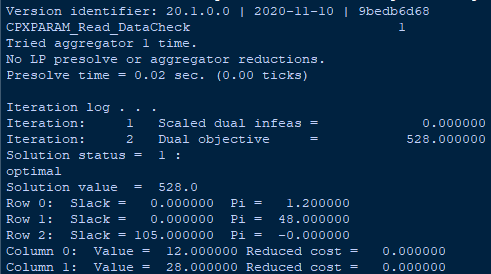
\includegraphics[width=10cm]{./images/Brasseur_Resolution.png}\label{Resultat_Brasseur}
 \caption{Résultat de l'optimisation du problème du brasseur}
 \end{center}
 \end{figure}

Nous voyons que nous avons pour revenu maximum 528 euro avec 12 unités de volume de bière blonde produite et 28 unités de volume de bière brune produites.

\subsection{Présentation de la résolution par backtracking}
L'algorithme du backtracking est plus précisément une famille d'algorithme qui sont utilisés le plus souvent pour résoudre des problèmes de satisfaction de contrainte.
Le backtracking est la solution la plus simple à comprendre il s'agit tout simplement de tester toutes les valeurs possible sur chaque case jusqu'a obtenir une sortie de sudoku remplie et valide.Cette algorithme agit comme un parcours d'arbre, illustrons cela avec une image:\newline

\begin{figure}[h]
  \begin{center}
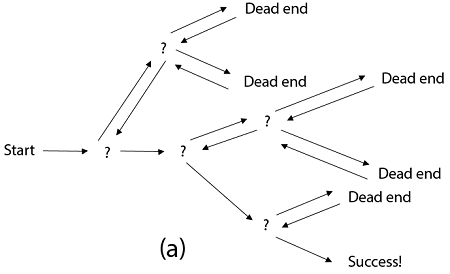
\includegraphics[width=10cm]{./images/backtracking.png}\label{Backtracking}
\caption{Illustration de l'algorithme du backtracking.}
\end{center}
\end{figure}

Comme l'illustre cette image nous essayons toutes les possibilitées et retournons en arrière si nous tombons dans une impasse dans notre cas, nous passons de case vide\footnote{\label{vide}Une case vide est comme dit plus haut une case contenant la valeur 0} en case vide\footref{vide} en revenant en arrière si peu importe le chiffre essayer dans cette case allant de 1 à 9, l'ajout de celui-ci donne un sudoku invalide. Le problème de cet algorithme qui reviens le plus souvent est dù au fait que nous essayons toutes les valeurs possible ce qui nous donne une très grande quantité d'action à éffectué et donc ce qui augmente considérablement notre temps de calcul nous pouvons toutefois régler ce problème en évitant de tester les possibilitées qui nous amène de façon logique à une impasse ou éviter de tester des possibilitées d'une case si il est possible de déduire sa valeur de façon logique.
\subsection{Pourquoi utiliser ces deux algorithmes}

\subsubsection{Pourquoi utiliser l'algorithme du simplex}

La résolution avec l'algorithme du simplex permet une implementation intuitive et facilité dù à l'utilisation de Cplex. Cplex nous permet aussi une meilleur étude de la complexité de notre algorithme car cous pouvons voir les différentes itération de recherche de notre outil de résolution. Cette méthode de résolution nous permet aussi de revoir le problème de plusieurs façons différentes de par le fait que la résolution ne dépends que de nos contraintes.

\subsubsection{Pourquoi utiliser l'algorithme utilisant le backtracking}

La résolution avec backtracking est l'algorithme le plus naturel qui viennent à l'esprit dans la résolution de problème avec contrainte ce qui permet une implémentation de la gestion des contraintes facilité malgré leur nombre.C'est un algorithme facilement améliorable car le but tout au long de son implémentation sera de tester le moins de valeur menant à une impasse possible. Cette algorithme a aussi pour avantage de n'avoir besoin d'aucune librairie extérieur ce qui permet une liberté totale au niveau du code et donne lieu à une certaine transparence quant à son fonctionnement contrairement au code que nous utilisons via cplex qui peut différé légèrement de son fonctionnement théorique.\newpage

\subsection{Implémentation des Stratégies de résolution}

\subsection{Modélisation et implémentation d'un sudoku en Python et de l'interface graphique}

\subsubsection{Présentation de l'interface graphique}
Nous allons tout d'abord vous présenter notre interface graphique qui nous servira tout au long de nos test:\newline

\begin{figure}[h]
  \begin{center}
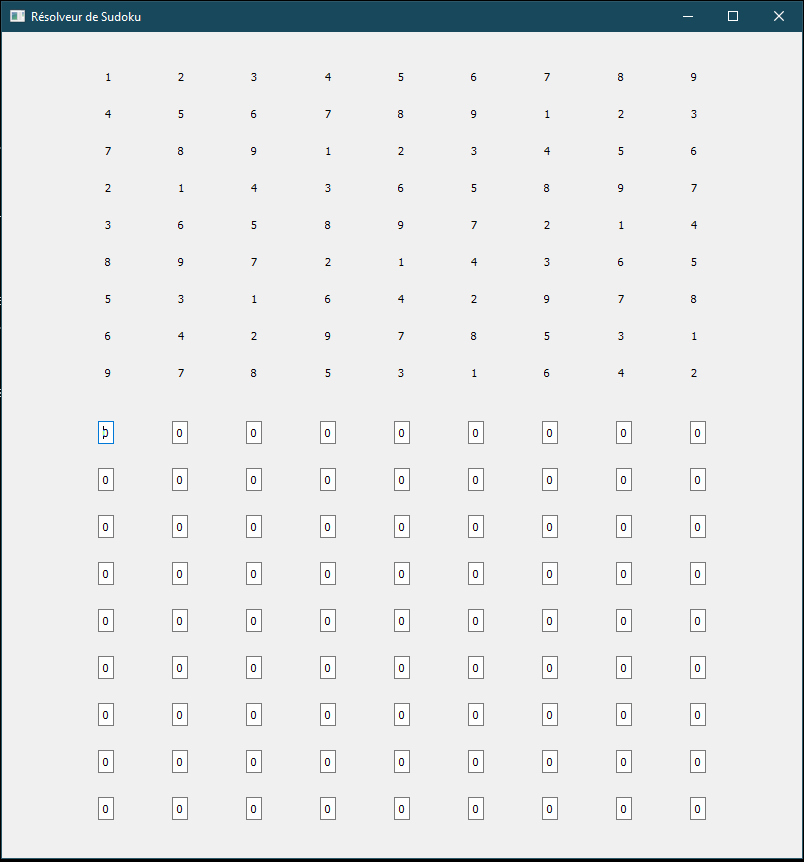
\includegraphics[width=8cm]{./images/Interface_Complete.png}\label{Interface_complete}
\caption{Interface graphique Complete.}
\end{center}
\end{figure}


\begin{figure}[h]
  \begin{center}
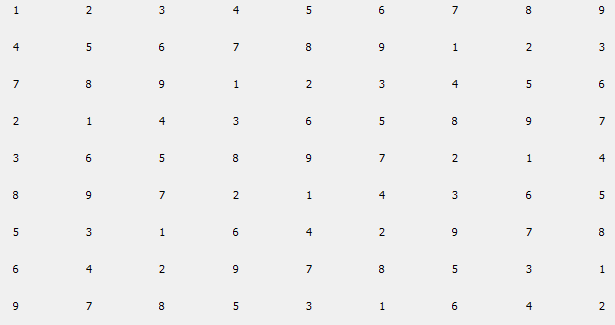
\includegraphics[width=8cm]{./images/Interface_Affichage.png}\label{Interface_affichage}
\caption{Zone d'affichage.}
\end{center}
\end{figure}


\begin{figure}[h]
  \begin{center}
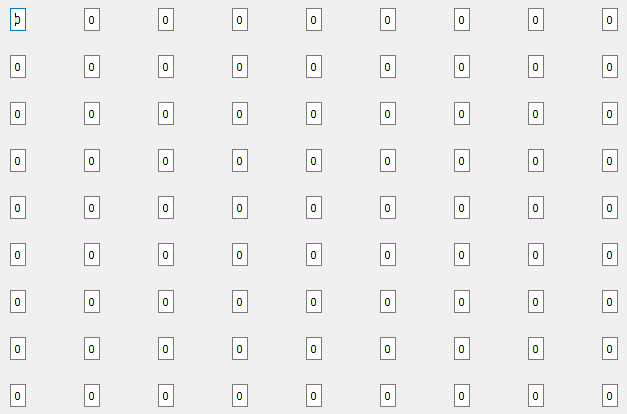
\includegraphics[width=8cm]{./images/Interface_saisi.png}\label{Interface_saisi}
\caption{Zone de saisi.}
\end{center}
\end{figure}

Notre interface se compose donc d'une zone de saisi qui contiendra le sudoku qui devra être résolu par notre programme et une zone d'affichage qui contiendra le sudoku une fois sa résolution par notre algorithme de résolution. L'affichage des nombres entrées dans la zone de saisi se fait de façon dynamique dans la zone d'affichage et la résolution se fait une fois que l'utilisateur a appuyé sur la touhe Entrée. Notre algorithme devant être innovant nous avons pensé à la généralisation du sudoku c'est à dire à ce que nous puissions choisir la taille des sudokus résolu par notre interface toujours avec un nombre de case et de ligne égales pour une raison d'impossibilité autrement à cause de la règle d'unicité sur les sous-grilles.\newline
Voilà donc notre interface avec un sudoku de 8 cases et 8 colonnes:\newline

\begin{figure}[h]
  \begin{center}
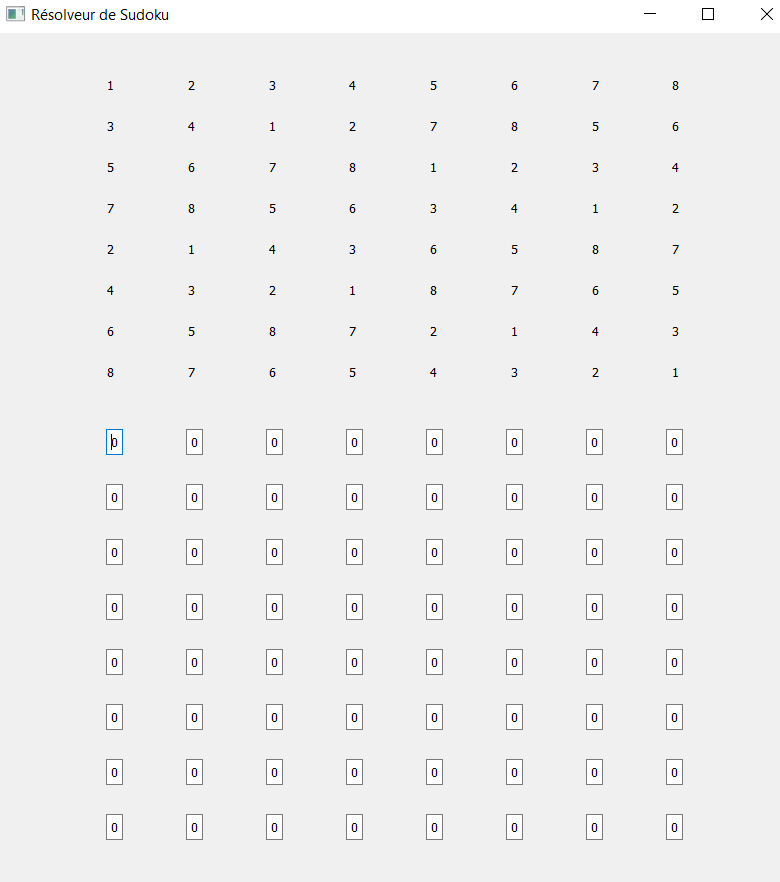
\includegraphics[width=8cm]{./images/8_8.png}\label{Interface_affichage_8_8}
\caption{Interface graphique de résolution d'un sudoku 8 par 8.}
\end{center}
\end{figure}


\subsubsection{Implémentation de l'interface graphique}

Nous allons stocker dans une liste\footnote{\label{liste_Python}structure de donnée incluse de base dans python qui permet de contenir plusieurs variables différentes} contenant 9 listes\footref{liste_Python} qui représenteront nos lignes qui elles contiendront 9 entiers allant de 0 à 9. Nous aurons donc besoin de coder des fonctions pour faire le lien entre l'interface et notre résolveur, du fait de notre modélisation du sudoku nous pouvons découper cela en plusieurs fonctions utilitaires:\newline
\begin{itemize}
\item Une fonction qui nous permettra de stocker le contenu de notre interface graphique dans une liste comme celle décrite précédemment.
\item Une fonction permettant de transférer le contenu d'une liste comme celle décrite plus haut dans la zone de saisi notre interface graphique.
\item Une fonction permettant de transférer le contenu d'une liste comme celle décrite plus haut dans la zone d'affichage notre interface graphique.
\item Une fonction permettant de copier le contenu de la zone de saisi de notre interface dans la zone d'affichage de notre interface.
\item Une fonction permettant de copier le contenu de la zone d'affichage de notre interface dans la zone de saisi de notre interface.
\end{itemize}

Pour la création de notre interface nous avons eu besoin de 3 panel\footnote{Contenant des différent élément de notre interface} un contenant nos deux grille nous permettant leur superpositon et deux qui sont nous servent de grilles car nos grilles ne sont en réalité que deux panel contenant un nombre de zone de saisi de texte aussi appelé QTextEdit dans la librairie Qt égale à la $taille^{2}$ et l'autre le même nombre de zone d'affichage de texte aussi appelé QLabel toujours dans la librairie Qt. Aussi nous avons eu besoin codés de quelques fonctions mineurs:\newline

\begin{itemize}
\item Une fonction nous permettant de faire en sorte que la taille des zones de saisi de textes soit calculé par rapport à ce qu'elle contiennent
\item Une fonction pour effectuerla résolution une fois la touche Entrée pressée.
\end{itemize}

\subsection{Implémentation de la résolution avec Cplex}

Comme nous l'avons fait dans notre exemple nous allons définir les contraintes et la fonction à maximiser:
Nous avons pour contrainte:
\begin{itemize}
\item La somme de chaque ligne doit être égal à 45 pour permettre l'utilisation de chaque chiffre sur une ligne
\item Les chiffres de chaques lignes doivent êtres différents
\item les chiffre de chaque colonnes doivent êtres différents
\item les chiffres de chaques sous grilles doivent être différents
\end{itemize}

Chaque inégalité peut être écrit sous la forme d'une fonction linéaire tel que:
\newline
$x-y=0$
\newline
La fonction à maximiser peut-être décrite comme la maximisation de la somme de chaque case en sachant que celle ci donnera toujours $9*45$ c'est a dire 405.
\newline
les case rempli c'est à dire les cases contenants les indices de notre sudoku peuvent êtres modélisé par une contrainte d'égalité en plus sur la variable représentant la case concerné.\newline
La généralisation du sudoku est implémenté telle qu'elle ne change pas la règle de l'unicité des chiffres sur les lignes et colonne et ne fait que fixer le nombre de valeur possible comme étant égale à la largeur ou longueur de notre sudoku car comme dit plus haut nous avons toujours le nombre de case sur une ligne égale au nombre de case sur une colonne. Nous pouvons donc décelé 2 cas a notre génération le meilleur cas ou le nombre n'est pas premier nous n'avons pour appliqué la règle des sous grilles qu'a trouvé un diviseur en privilégiant un diviseur dont le résultat de la division donne lui même ainsi notre sous grille pour le cas d'une résolution 10 ligne par 10 colonnne par exemple considéré que les sous grilles ce compose de 2 élémment sur les grilles et 5 élément sur les colonnes:

\begin{figure}[h]
  \begin{center}
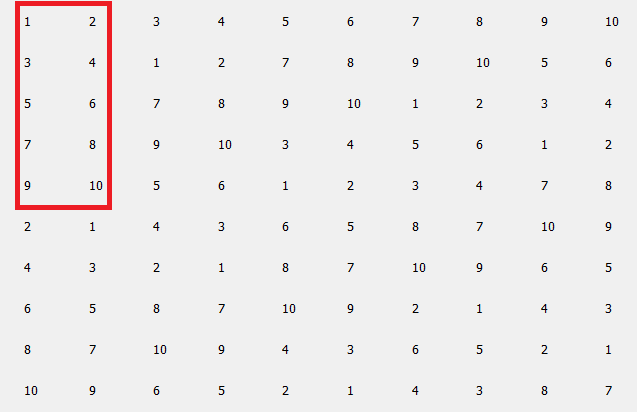
\includegraphics[width=8cm]{./images/10_10.png}\label{10_10}
\caption{Sudoku 10 par 10 résolu montrant la première sous grille.}
\end{center}
\end{figure}

\subsection{Implémentation de la résolution avec l'algorithme du backtracking}

Pour cette algorithme nous avons besoin de 4 fonctions très simple:

\begin{itemize}
  \item Une fonction pour copier notre liste.
  \item Une fonction pour vérifier si notre sudoku est toujours valide autrement dit respect nos contraintes.
  \item Une fonction pour vérifier si notre sudoku est remplie autrement dit ne cotient pas de case contenant la valeur 0.
  \item Notre fonction principale qui utilisera toute les autres pour résoudre notre sudoku.
\end{itemize}

\subsubsection{Première fonction}

Cette fonction nous sera utile a car en cas d'érreur quand nous testons les valeur nous devons pouvoir retourner en arrière et donc nous devons garder le sudoku de l'itération de test précédente, c'est pour cela que pour chaque test de valeur nous utiliserons une copie du sudoku de l'itération précédente.\newline

\subsubsection{Deuxième fonction}

Cette fonction doit vérifier nos différentes règles d'unicité et si ls valeur des différente cases sont belle et bien comprises entre 1 et la largeur et longueur du sudoku. Elle doit considéré un sudoku incomplet mais respectant toutes les contraintes comme étant un sudoku valide car dans le cas contraire aucune valeur testée sur la première case vide si il y en a d'autre ne serait valide ce qui nous empêcherait d'avancer dans nos test.\newline

\subsection{Troisième fonction}

Comme dit précédemment nous considèrons un sudoku incomplet mais respectant nos contraintes d'unicité comme étant valide. Nous avons donc besoin dune fonction pour savoir si notre sudoku est rempli ou non pour terminer notre résolution. Un sudoku résolu étant un sudoku remplie et valide.\newline

\subsection{Fonction principale}

Cette fonction est la plus longue de notre programme de résolution mais n'en est pas moins simple cette fonction doit en premier lieu trouver la première case vide dans le sens de lecture de notre sudoku (de gauche a droite et de haut en bas).\newline
Puis doit tester les valeur de 1 à 9 en faisant attention avant de tester une valeur de vérifier si le sudoku est toujours valide si elle est posé avant de l'essayer.\newline
Une fois une valeur valide trouver la fonction on répète cette opération defaçon récursive\footnote{Par un appelle de la fonction dans cette même fonction} mais cette fois avec notre copie de sudoku avec notre nouvelle valeur ajoutée.\newline
Si nous ne trouvons aucune valeur de 1 à 9 pour notre case nous retournons la liste sans ajouté de valeur afin de tester une autre valeur dans la case vide précédente.\newline
Comme dit précédemment nous ne nous arrêtons que quand notre sudoku est remplie et valide.\newline

\section{Test du résolveur}

\subsection{Choix de nos test}

\subsubsection{Test avec un sudoku standart complètement vide}

Nous avons tout d'abord pensé à essayer notre résolveur sur un sudoku complètement vide, ce sudoku ayant le plus grand nombre de solution car à ce sudoku est solution toutes les grilles de sudoku existantes, s'agit donc d'un des meilleurs cas possible pour nos deux algorithmes.

\subsubsection{Test avec un sudoku standart rempli de 17 valeurs}

Maintenant que nous avons identifié notre meilleur des cas commun nous pouvons maintenant essayer de trouver notre pire des cas commun, c'est grace a un article que nous avons pu l'identifier en effet selon cette article: \cite{NombredeDieu}\newline
Nous avons appris que Le nombre minimal d'indicepour n'avoir qu'une seule solution a une grille de sudoku était 17. Ce qui en plus de n'admettre qu'une seule solution possible nous donne le moins de valeur déjà entrer possible.

\subsection{Test de la généralisation}

Quand aux sudoku de taille différente nous n'avons qu'éffectuer des sudoku sans indices de par le fais de notre méconnaissance de ceux-ci car contrairement au sudoku standart nous n'avons pas trouver d'équivalent au nombre de dieu des sudoku standart et n'avons pas les moyen d'en éffectuer la recherche comme il a été fait dans l'article.

\subsection{Implémentation de nos test}

Nous n'avons eu besoin pour l'implémentation de nos test que d'une liste contenant des 0 pour notre cas le plus simple. Et pour notre cas le plus compliqué nous avons choisi de télécharger un fichier contenant 9 000 000 de sudoku résolu et n'avons eu qu'a en enlevé 64 valeurs et avons essayé notre sudoku sur quelque un d'entre eux.

\subsection{Résultat de nos tests}
\subsubsection{Changement d'algorithme de cplex}
Nos test avec les sudoku standart nous ayant mené a la conclusion que l'algorithme du simplex nous menant à un temps de résolution bien trop long dans les deux cas nous avons finaleent utiliser l'optimiseur de cplex utilisant un autre algoritme de résolution mais ne changeant pas l'implémentation mais changeant légèrement nos contrainte nous avons donc utiliser la contrainte Alldiff de cplex pour les différentes règles d'unicité ayant une bien meilleur éfficacité, et remplacer la contraintes de la somme des valeur d'une ligne par une contraintes de valeur sur chaque variables pour qu'elles ne varient qu'entre 1 et 9.
\newpage
\subsection{résultat avec notre nouvelle algorithme}
Nous avons une réponse quasi instentanées dans les tout les cas, voilà les résultats de nos différentes résolutions:

\begin{figure}[h]
  \begin{center}
\includegraphics[width=8cm]{./images/Res_Vide.png}\label{Test_Cplex}
\caption{Résolution de Grille Vide avec l'optimizer de Cplex.}
\end{center}
\end{figure}

\begin{figure}[h]
  \begin{center}
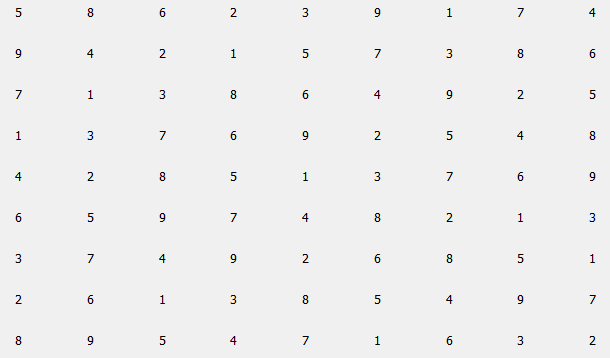
\includegraphics[width=8cm]{./images/Res_17.png}\label{Test_Cplex_17}
\caption{Résolution de Grille avec 17 indices grace à l'optimizer de Cplex.}
\end{center}
\end{figure}


\begin{figure}[h]
  \begin{center}
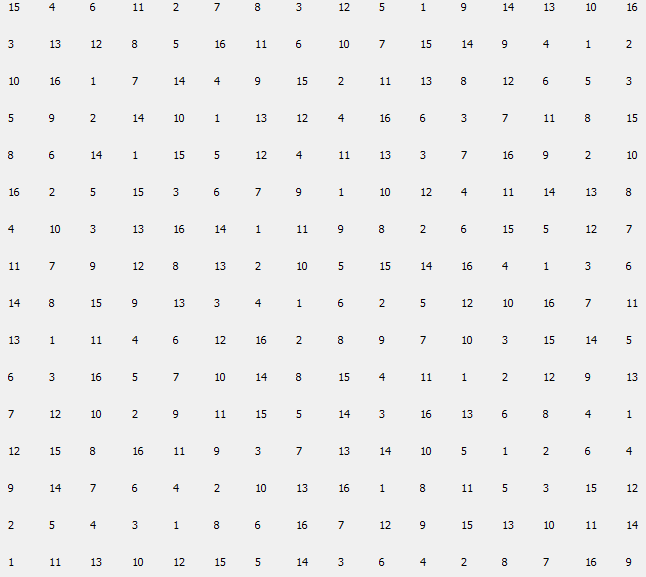
\includegraphics[width=8cm]{./images/Resultat_16_Cplex.png}\label{Test_Cplex_16_16}
\caption{Résolution de Grille de longueur et largeur égale à 16 grace à l'optimizer de Cplex.}
\end{center}
\end{figure}
\newpage
\subsection{Résultat avec notre algorithme de BackTracking}
Pour ce qui est de l'algorithme utilisant le backtracking nous avons dans les deux cas avec des sudoku standart des réponses instantanées. Pour ce qui est du résultat avec un sudoku généralisé de taille 16 par 16 nous avons un temps de réponse notable et assez génant voir beaucoup trop long pour certaines tailles tel que 15.\newline
Voila les résultats de nos résolutions:

\begin{figure}[h]
  \begin{center}
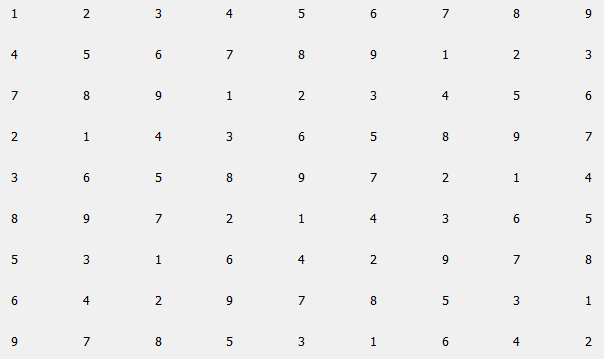
\includegraphics[width=8cm]{./images/Res_Back_Vide.png}\label{Test_Back}
\caption{Résolution de Grille Vide avec l'algorithme utilisant le backtracking.}
\end{center}
\end{figure}


\begin{figure}[h]
  \begin{center}
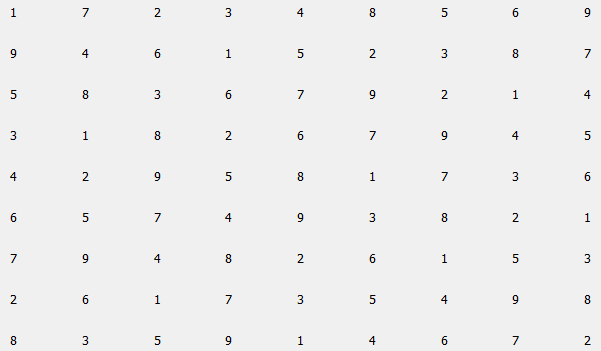
\includegraphics[width=8cm]{./images/Res_Back_17.png}\label{Test_Back_17}
\caption{Résolution de Grille avec 17 indices avec l'algorithme utilisant le backtracking.}
\end{center}
\end{figure}


\begin{figure}[h]
  \begin{center}
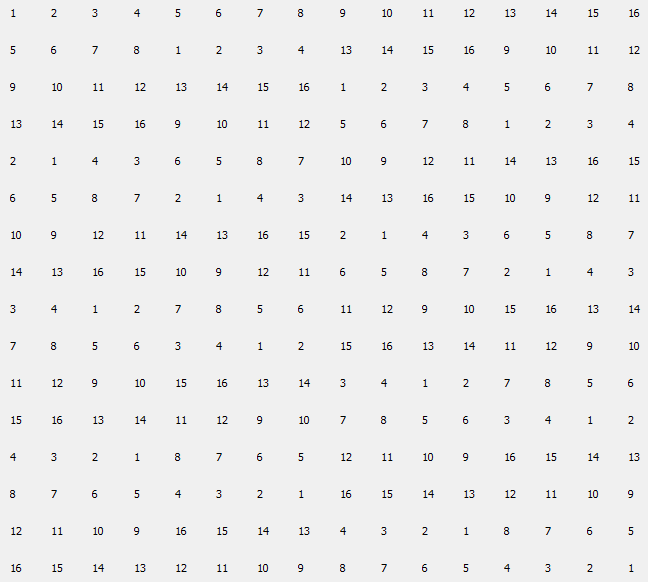
\includegraphics[width=8cm]{./images/Resultat_16_Back.png}\label{Test_Back_16_16}
\caption{Résolution de Grille de longueur et largeur égale à 16 avec l'algorithme utilisant le backtracking.}
\end{center}
\end{figure}

\subsection{Analyse de nos résultats}

\subsubsection{Résultats avec Cplex}

Les résultats de l'utilisation de Cplex sont extrèmement positif pouvant réaliser des tailles extrèmes de sudoku sans aucun problème.

\subsubsection{Résultat avec l'utilisation de BackTracking}

Les résultats avec l'utilisation du backtracking permettent parfaitement de résoudre un sudoku standart peu importe les indices données et leur nombre. Mais la généralisation laissant a désiré nous pouvons réfléchir à plusieurs piste d'amélioration de cela nous pouvons par exemple pour améliorer l'éfficacité de notre algorithme, éviter les configurations où les valeurs peuvent êtres déduites de façon logique tel que celui ci:

\begin{figure}[h]
  \begin{center}
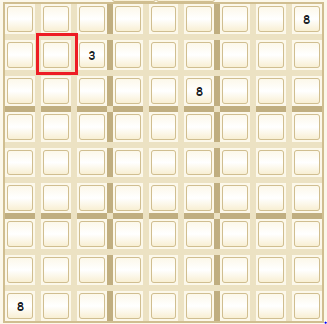
\includegraphics[width=8cm]{./images/Exemple_deduction.png}\label{Exemple_Logique}
\caption{Exemple de case dont la valeur peut-être déduite de façon logique dans notre cas la valeur dans la case encadré est 8.}
\end{center}
\end{figure}
